\documentclass[10pt,a4paper,]{article}
\usepackage[a4paper,margin=2.5cm]{geometry}
\usepackage{graphicx}
\usepackage{setspace}
\usepackage{sectsty}
		\allsectionsfont{\bfseries\normalsize} % section header sizes \sffamily

\usepackage{lmodern}

\usepackage{xcolor}
\usepackage{colortbl}

\usepackage[labelfont=bf]{caption}
\captionsetup{margin=1cm}
		% \captionsetup{justification=centering} % or font=small, labelfont=bf etc.
		% \setlength{\abovecaptionskip}{5pt} % caption offset
		% if captions are too long for a table, squeeze their space by \captionsetup{margin=2cm} inside the local environment (e.g. table)

\renewenvironment{quote}
  {\list{}{\rightmargin=0cm \leftmargin=.5cm}%
   \item\relax}
  {\endlist}

\usepackage{setspace}
\setstretch{1.15}

\skip\footins 20pt plus4pt minus4pt
\setlength{\footnotesep}{10pt}
\usepackage[hang,flushmargin]{footmisc}\renewcommand{\footnotemargin}{\ifnum\value{footnote}<10 5pt \else 9pt\fi}

\clubpenalty = 10000
\widowpenalty = 10000
\displaywidowpenalty = 10000


% \newlength{\cslhangindent}
% \setlength{\cslhangindent}{1.5em}
% \newenvironment{cslreferences}%
%   {\setlength{\parindent}{0pt}%
%   \everypar{\setlength{\hangindent}{\cslhangindent}\setlength{\parskip}{0pt}}\ignorespaces}%
%   {\par}




% \usepackage[compact]{titlesec} % left margin, above-skip and below-kip
% \titlespacing{\section}{0pt}{8pt}{0pt}
% \titlespacing{\subsection}{0pt}{8pt}{0pt}
% \titlespacing{\subsubsection}{0pt}{6pt}{-3pt}
% \titlespacing{\subsubsubsubsection}{0pt}{3pt}{-3pt}
% % \titlespacing{\subsubsubsubsection}{0pt}{3pt}{-3pt}
% \titleformat{\subsubsubsubsection}[runin]{\normalfont\bfseries}{\S\ \thesection.}{.5em}{}[. ]
% \titlespacing{\subsubsubsubsection}{\parindent}{1.5ex plus .1ex minus .2ex}{0pt}
% \renewcommand{\subsubsubsection}{\paragraph}

\usepackage{amssymb,amsmath}
\usepackage{ifxetex,ifluatex}
\usepackage{fixltx2e} % provides \textsubscript
\ifnum 0\ifxetex 1\fi\ifluatex 1\fi=0 % if pdftex
  \usepackage[T1]{fontenc}
  \usepackage[utf8]{inputenc}
\else % if luatex or xelatex
  \usepackage{unicode-math}
  \defaultfontfeatures{Ligatures=TeX,Scale=MatchLowercase}
    \setmainfont[]{Libertinus Serif}
\fi
% use upquote if available, for straight quotes in verbatim environments
\IfFileExists{upquote.sty}{\usepackage{upquote}}{}
% use microtype if available
\IfFileExists{microtype.sty}{%
\usepackage[]{microtype}
\UseMicrotypeSet[protrusion]{basicmath} % disable protrusion for tt fonts
}{}
\PassOptionsToPackage{hyphens}{url} % url is loaded by hyperref
\usepackage[unicode=true]{hyperref}
\hypersetup{
            pdftitle={A simple template for gdoc},
            pdfauthor={Yingqi Jing\^{}\{1,2\}; Author Two\^{}3 and Author Three\^{}1},
            pdfkeywords={word order, linguistic typology, language evolution},
            pdfborder={0 0 0},
            breaklinks=true}
\urlstyle{same}  % don't use monospace font for urls
\usepackage{longtable,booktabs}
\usepackage{multirow}
% Fix footnotes in tables (requires footnote package)
\IfFileExists{footnote.sty}{\usepackage{footnote}\makesavenoteenv{long table}}{}
\IfFileExists{parskip.sty}{%
\usepackage{parskip}
}{% else
\setlength{\parindent}{0pt}
\setlength{\parskip}{6pt plus 2pt minus 1pt}
}
\setlength{\emergencystretch}{3em}  % prevent overfull lines
\providecommand{\tightlist}{%
  \setlength{\itemsep}{0pt}\setlength{\parskip}{0pt}}
\setcounter{secnumdepth}{5}
% Redefines (sub)paragraphs to behave more like sections
\ifx\paragraph\undefined\else
\let\oldparagraph\paragraph
\renewcommand{\paragraph}[1]{\oldparagraph{#1}\mbox{}}
\fi
\ifx\subparagraph\undefined\else
\let\oldsubparagraph\subparagraph
\renewcommand{\subparagraph}[1]{\oldsubparagraph{#1}\mbox{}}
\fi

% set default figure placement to htbp
\makeatletter
\def\fps@figure{htbp}
\makeatother

% gloss formatting
\usepackage{gb4e,cgloss4e}
\let\eachwordone=\itshape
\let\eachwordtwo=\small
\def\gltoffset{0.5ex}

\usepackage{standalone}
\usepackage{threeparttablex}
\usepackage{longtable}
\usepackage{amsmath}
\usepackage{caption}
\usepackage{subcaption}
\usepackage{upgreek}
\usepackage{float}
\usepackage{multirow}

\title{A simple template for gdoc\thanks{We would like to thank.}}
\author{Yingqi Jing\(^{1,2}\) \and Author Two\(^3\) and Author Three\(^1\)}
\date{}

\begin{document}
\thispagestyle{empty}
% \maketitle

\begin{center}
{\doublespacing
{\Large\sffamily\bfseries{A simple template for gdoc}}\\[6pt]

{\normalsize Yingqi Jing\(^{1,2}\), Author Two\(^3\) and Author Three\(^1\)}
\\ % \sf
}
{\vspace{\baselineskip}\small \(^1\)Department of Language and Philology, Uppsala University, \(^2\)Department of Comparative Language Science, University of Zürich, \(^3\)Department of Basic Neuroscience, University of Geneva}



\end{center}
\vspace{6pt}


\vspace{\baselineskip}
\begin{abstract}
This is the abstract! This is the abstract of the paper. An abstract
summarizes, usually in one paragraph of 300 words or less, the major
aspects of the entire paper in a prescribed sequence that includes: 1)
the overall purpose of the study and the research problem(s) you
investigated; 2) the basic design of the study; 3) major findings or
trends found as a result of your analysis; and, 4) a brief summary of
your interpretations and conclusions.
\end{abstract}\vspace{2\baselineskip}

\setlength{\parskip}{4pt} \renewcommand{\labelitemi}{-} \clubpenalty =
10000 \widowpenalty = 10000 \displaywidowpenalty = 10000

\let\eachwordone=\itshape
\let\eachwordtwo=\small
\def\gltoffset{0.5ex}

\section{Introduction}\label{introduction}

This is an introduction (Kemmerer
\protect\hyperlink{ref-Kemmerer2012}{2012}).

\begin{exe} \ex Expectation-based facilitation in German \label{ex-german}
\begin{xlist}
\ex \gll Er hat das Buch, [das Lisa gestern gekauft hatte], hingelegt.\\
         he has the book that Lisa yesterday bought had laid.down\\
\ex  \gll Er hat das Buch hingelegt, [das Lisa gestern gekauft hatte].\\
        he has the book laid.down that Lisa yesterday bought had\\
       \glt ‘He has laid down the book that Lisa had bought yesterday.’ 
\end{xlist}
\end{exe}

In self-paced reading, the verb is read faster in such examples when it
follows the semantically rich and complex noun phrase in
\ref{ex-german}a (``the book that Lisa bought yesterday'') than when it
follows the short object noun phrase ``the book'' in \ref{ex-german}b,
where the relative clause is extraposed. Since these facilitation
effects matter most for long and information-rich dependents, one would
expect less variation in placement with longer dependencies
(long→head-final→less variable).

\section{Data and Methods}\label{data-and-methods}

This is the section for data and methods. The information of these
treebanks is summarized in Table \ref{tab:UD-data}.

\begin{center}
\setlength\tabcolsep{2pt}
\begin{ThreePartTable}
\footnotesize
\begin{longtable}[h]{llcrr|llcrr}
\caption{Overview of 71 dependency treebanks from UD v2.7.\label{tab:UD-data}} \\
\hline
\endfirsthead
\toprule
\endhead
\vspace{-0.05cm}
Language & Family & Europe & Sentences & Word token & Language & Family & Europe & Sentences & Word token\\
\midrule
Afrikaans & Indo-European & F & 1,934 & 49,276 & Irish & Indo-European & T & 4,910 & 115,969\\
Akkadian & Afro-Asiatic & F & 1,804 & 21,962 & Italian & Indo-European & T & 14,167 & 298,343\\
Ancient Greek & Indo-European & T & 17,080 & 213,999 & Japanese & Japanese & F & 57,028 & 1,250,875\\
Arabic & Afro-Asiatic & F & 19,738 & 738,889 & Korean & Korean & F & 27,363 & 350,090\\
Armenian & Indo-European & T & 2,502 & 52,630 & Latin & Indo-European & T & 26,977 & 450,515\\
Bambara & Mande & F & 1,026 & 13,823 & Latvian & Indo-European & T & 13,643 & 219,955\\
\bottomrule
\end{longtable}
\end{ThreePartTable}
\end{center}

We predict the direction and variation of each word order in a model
assuming a Beta-Binomial likelihood function. The Beta-Binomial
distribution is a mixture of a Binomial and a Beta
distribution.\footnote{This is my footnote.} It generalizes the Binomial
distribution, and can capture overdispersion. With the Beta-Binomial
model, the Binomial probability is randomly drawn from a Beta
distribution \(\mathbf{B}\left(\alpha, \beta \right)\) with
hyperparameters \(\alpha > 0\) and \(\beta > 0\).

\begin{equation*}
\text{Beta2} \left(\mu, \phi \right) = \text{Beta} \left(\alpha = \frac{\mu}{\phi}, \beta = \frac{\left(1 - \mu \right)}{\phi} \right)
\end{equation*}

\section{Results}\label{results}

You can put some fancy results here! Figure \ref{fig-raw-dist}
visualizes the relationship.

\captionsetup{margin=1cm}

\begin{figure}[htpb]
\centering
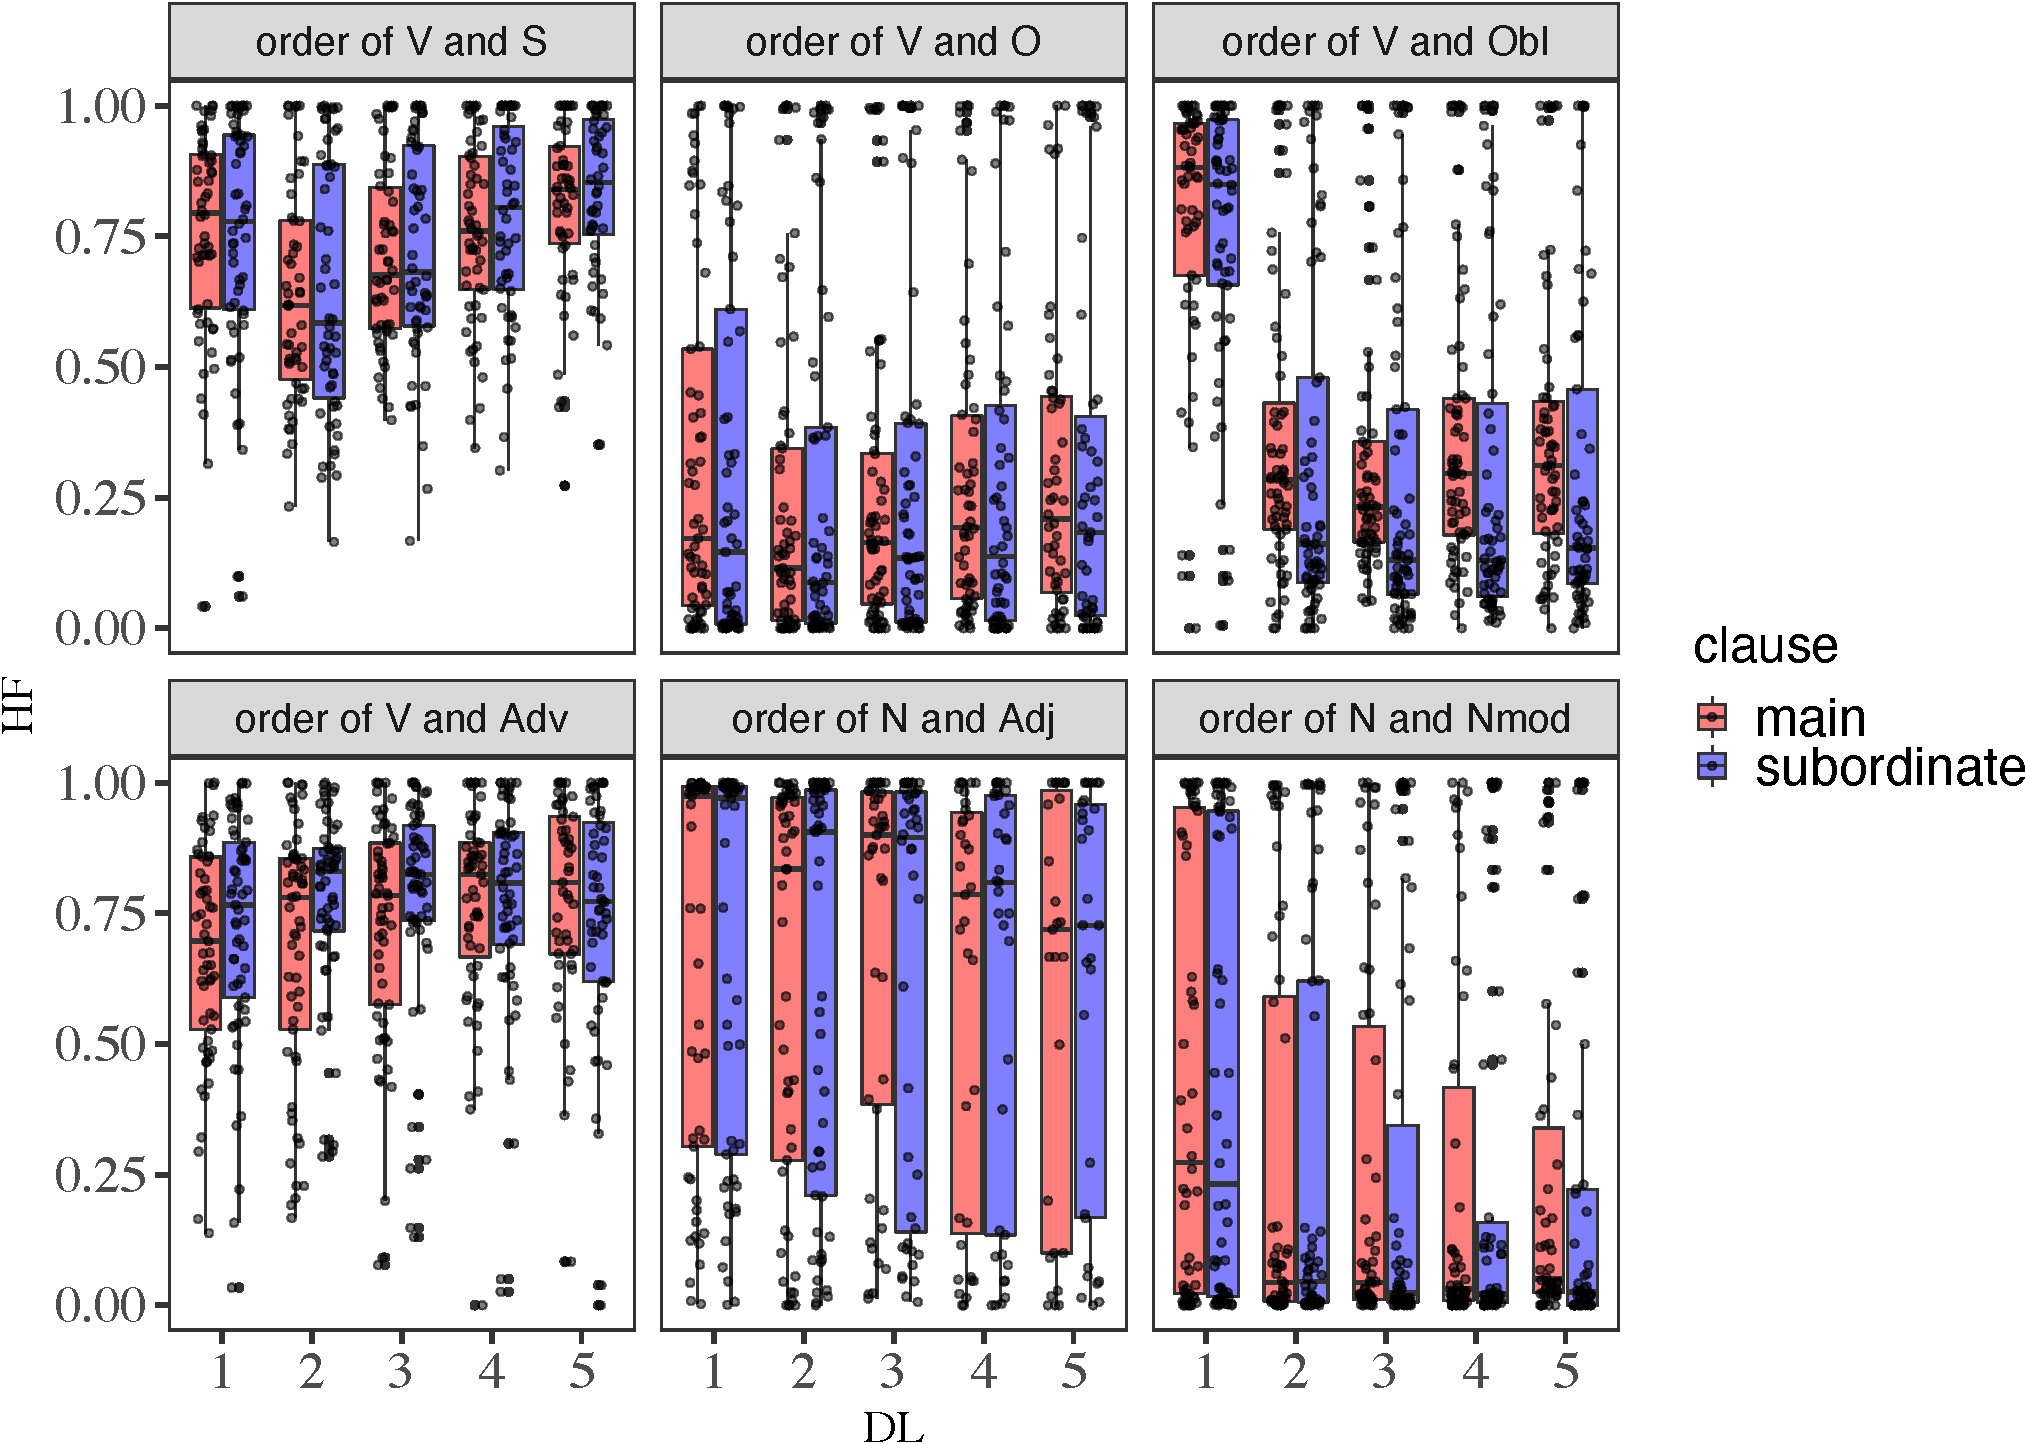
\includegraphics[width=14cm, height=10cm]{figures/relationship between DL and HF-1.pdf}
\caption{Boxplots for the distribution of raw head-final (HF) dependencies in relation to dependency length (DL) across main and subordinate clauses} 
\label{fig-raw-dist}
\end{figure}

\section{Conclusion}\label{conclusion}

Here is the conclusion. \setlength{\parskip}{0pt} \raggedright
\setstretch{1}

\section*{References}\label{references}
\addcontentsline{toc}{section}{References}

\hypertarget{refs}{}
\hypertarget{ref-Kemmerer2012}{}
Kemmerer, David. 2012. The Cross-Linguistic Prevalence of SOV and SVO
Word Orders Reflects the Sequential and Hierarchical Representation of
Action in Broca's area. \emph{Language and Linguistics Compass} 6.
50--66.

%TC:endignore
\end{document}
